\documentclass[12pt]{article}
%Gummi|065|=)
\usepackage{amsmath, amsfonts, amssymb}
\usepackage[margin=0.5in]{geometry}
\usepackage{xcolor}
\usepackage{graphicx}

%\usepackage{pifont}
\usepackage{amsmath}

\newcommand{\off}[1]{}
\DeclareMathSizes{20}{30}{20}{18}

\newcommand{\two }{\sqrt[3]{2}}
\newcommand{\four}{\sqrt[3]{4}}
\newcommand{\red}{\begin{tikz}[scale=0.25]
\draw[fill=red, color=red] (0,0)--(1,0)--(1,1)--(0,1)--cycle;\end{tikz}}
\newcommand{\blue}{\begin{tikz}[scale=0.25]
\draw[fill=blue, color=blue] (0,0)--(1,0)--(1,1)--(0,1)--cycle;\end{tikz}}
\newcommand{\green}{\begin{tikz}[scale=0.25]
\draw[fill=green, color=green] (0,0)--(1,0)--(1,1)--(0,1)--cycle;\end{tikz}}

\newcommand{\sq}[3]{\draw[#3] (#1,#2)--(#1+1,#2)--(#1+1,#2+1)--(#1,#2+1)--cycle;}

\usepackage{tikz}

\newcommand{\susy}{{\bf Q}}
\newcommand{\RV}{{\text{R}_\text{V}}}

\title{Scratchwork: Geometry of Numbers}
\date{}
\begin{document}

%\fontfamily{qag}\selectfont \fontsize{12.5}{15}\selectfont

\sffamily

\maketitle

\noindent As I read attempting to read Manjul Bhargava's papers, a few problems emerge:
\begin{itemize}
\item I don't know some of the groups definitions that he refers to
\item I don't know what he is calling ``geometry of numbers"
\item I don't know what the big deal is about class numbers.  Or why his contrubtions were so crucial.
\end{itemize}
Geometry of Numbers has been around since Hermann Minkowski, and there's even the book, written in academic 19th century German \textit{Geometry der Zahlen}.  And who knows?  Perhaps that bounds have improved since then, \dots there is the book of Cassels in the mid 20th century.  This area - when I learned it - amounted to a ``cute proof" that should be solve using more robust methods - and then Manjul won a Field's medal with it in 2014.\footnote{1) that is my personal opinion, and usually when you ask someone suddenly everyone changes their position \dots 2) I have look at him in person, maybe one or two-odd times in my life. }\\ \\
The geometry of numbers proof (e.g. Davenport) that $n = a^2 + b^2 + c^2 + d^2$ uses lattices over $\mathbb{R}^4$. However the proof that $p = 4k+1 = a^2 + b^2$ uses a mix of mod $p$ arithmetic -- over $(\mathbb{Z}/p\mathbb{Z})^2$ to define (an essentially random) lattice over $\mathbb{R}^2$.  So, we are going to combine the two objects. \\\\
At this point $p$ is still generic, so it's safe to say we are solving the ``family" equations $x^2 + y^2 = n$ \textbf{at all primes p}.
$$ X = \{ x^2 + y^2 - n = 0 \} \to \big( \mathbb{Z}/p\mathbb{Z} \times \mathbb{R} \big)^2 $$
and we are looking for lattices in this mixed geometirc object.  And if we have $X(\mathbb{Z}/p\mathbb{Z})$ and $X(\mathbb{R})$ we could even have:
$$ X(\mathbb{Z}_p) \to \dots \to X(\mathbb{Z}/p^{k+1}\mathbb{Z}) \to X(\mathbb{Z}/p^k \mathbb{Z}) \to \dots \to X(\mathbb{Z}/p \mathbb{Z})  $$
While looking at the scheme $X(\mathbb{Z})$ at one place $p$ is not enough if we look at a generic place $p$ \textit{as well as} $p = \infty$ we can have
$$ X(\mathbb{Z}) ``\simeq" X(\mathbb{Z}_p) \cap X(\mathbb{R})$$
and maybe this is sufficient.  \\ \\
Even if you know and prove Fermat's result that $p = 4k+1$ prime is the sum of two squares what have you gained from that:
$$ p = a^2 + b^2 = (a+bi)(a-bi) \text{ then } a+bi \in \sqrt{a^2 + b^2}\,e^{i\theta} $$
so there is an angle, $\theta$ that's unpredictiable.  In more modern language we could say that primes in $\mathbb{Z}[i]$ are rotationally symmetric in large scale.  \\ \\
There are two good exampls of Fermat's descent:
\begin{itemize}
\item $p = a^2 + b^2$
\item $\sqrt{2} \notin \mathbb{Q}$
\end{itemize}
\newpage 
\noindent Wikipedia (and other books) indicate that descent can be considered a type of Galois Cohomology.  Since a result like this is ``clear" from elementary means, why should you build it from this complicated machinary?  Here's the basic argumen:
$$ x^2 = 2y^2 \to x = 2z \to (2z)^2 = 2y^2 \to 2z^2 = y^2 \to y^2 = 2z^2 $$ 
The rest of the steps amound to identifying a variety (or scheme) basically the equation we are trying to solve, and the appropriate cohomology groups.
$$ X = \{  x^2 - 2y^2  = 0 \}$$
That is the equation we are trying to solve.  Now it's our variety or Scheme.  We could consider $X(\mathbb{Z})$ or $X(\mathbb{Q})$ or $X(\mathbb{Q}_p)$ or whatever.  All these equations we just calculated can be summarized by saying we found a \textbf{map}. 
$$ T: X \to X \text{ with } (x,y) \mapsto (y, x/2)$$
Then we say something interesting... we say our solution has gotten ``smaller", e.g.
$$ x^2 + y^2 > y^2 + (x/2)^2 \in \mathbb{Z} $$
In what sense have our solutions gotten smaller?  We are not longer just using a field, we are using an \textit{ordered} field, either $\mathbb{Q}$ or $\mathbb{R}$:
\begin{eqnarray*} X(\mathbb{Z}) = \{  x^2 - 2y^2  = 0 \} &\subseteq&  X(\mathbb{Q}) =
\{  x^2 - 2y^2  = 0 \} \\ 
&\subseteq & X(\mathbb{R})
= \{ (x - \sqrt{2}y)(x + \sqrt{2}y) = 0 \} 
= \{  x- \sqrt{2}y = 0 \} \cap \{  x+ \sqrt{2}y = 0 \} \end{eqnarray*}
and finally we say that there are no infinitely descending sequences of integers. \\ \\
In a way, we have done nothing.  And we can go even futher .  We might do this when the elementary means are unavailable, and when our own sense fail us or lead us astray.  Now we consider $x$ as a \textit{function}:
$$ x, y : X(\mathbb{Z}) \to \mathbb{Z} \text{ so that } x, y \in H^1(X, \mathbb{Z})$$
I'm not sure if this is the torsor that the Number Theorists use.  In fact, they use 
$$ H^1(k, G) \text{ possibly } H^1(\mathbb{Q}, T) $$
setting $k = \mathbb{Q}$ and $G = \{ T^k: k \in \mathbb{Z}\}$ to be iterations of the `` $\times$2 " map we discussed.  Then the idea of local-to-global is that we find a solution over $k$ if we solve over all completions $k_v$:
$$ \text{if }[X]= 0 \in H^1(k_v, G) \text{ then }[X]=0 \in H^1(k, G) $$
or we could state it as some type of product
$$ H^1(k, G) \to \prod_v H^1(k_v, G) $$
In our case $k = \mathbb{Q}$, $[X] = \{  x^2 - 2y^2 = 0\}$ and $G $ is basically the map $(x,y) \mapsto (y/2, x)$.  This amonunts to saying that for two relatively prime numbers $m, n \in \mathbb{Z}$ we could try to solve by unique factorization.
$$  $$
All these homology theories are (sometimes useful) layers that we put over real calculations and real things that are happening.  There is a torsor cohomology $H^1(X, G)$ where we could discuss classes of torsors\footnote{Can't they just say ``group action"?} over $X$. \'{E}tale cohomology over $\mathrm{Spec} k$ is Galois cohomology, so we could stop here and I will. \\ \\
We ought to discuss $p = a^2 + b^2$ a bit (btw I'm using notes of Brian Conrad on desent).

\newpage

\noindent \textbf{09/28} Let's try to read one of Manjul's abstracts:
\begin{quotation}
We develop {\color{blue!50!gray}geometry-of-numbers} methods to count orbits in \textbf{prehomogeneous vector spaces}
having bounded invariants over any global field. As our primary example, we apply these techniques to determine, for any base global field F of characteristic not 2, the {\color{red!50!gray}density of discriminants} of field extensions of degree at most 5 over $F$.
\end{quotation}

No idea\dots Let's try reading the first page.  Or two: 
\begin{quotation}
Let F denote a global number or function field. A fundamental problem in arithmetic statistics
is to determine the densities of discriminants of field extensions of F having a fixed degree n over F.
The case of $n = 2$ when $F = \mathbb{Q}$ (and the case of $n = 1$ for all F!) are trivial. When $n = 3$, even the
case $F = \mathbb{Q}$ is highly nontrivial and is a celebrated result of Davenport-Heilbronn [29]. Surprisingly,
even the case $n = 2$ is nontrivial for more general F and is a result of Datskovsky-Wright [27], who
also settle the case of $n = 3$ for general global fields F having characteristic not 2 or 3. The cases $n = 4$
and 5 for $F = \mathbb{Q}$ were carried out in [6, 7].
\end{quotation}
and then it hit me.  Do I have the same concerns as Manjul?  That's unlikely.  I hardly know the guy nor his style of mathmatics.  OK.  Are these two problems the same?
\begin{itemize}
\item density of discriminants 
\item sum of squares, $p = a^2 + b^2$
\end{itemize}
The second question ``Fermat's theorem" has evolved to the question of whether a prime $\mathfrak{p}$ splits in a given field, $L$.  The culmination of Abelian class field theory the Kronecker-Weber theorem is no longer a statement about diophantine equations - an equation with numbers in it... In fact I don't really know what it says. \\ \\ 
The discriminant question merely asks about various extensions $F \subseteq L$ with $[L:F] = 2 \text{ or } 3$.  How can we index all the number fields $L$ that extend $F$?  And then we'd have to reason about the Galois groups of each of them, or mentally sort them by Galois group.\\ \\
There's a bit of a social problem I'll just outline: within mathematics (ignoring 90\% of the world) the fraction of people \textit{learning} Class Field Theory is quite small.  Either they know it or they don't.  The number of fraction learning Elementary Number Theory is quite large; there's always somebody (this could be overestimate).  So\dots Class Field Theory no longer looks like baby math.  It could, but nobody does the conversion.  Maybe it's too complicated to write down.\footnote{We can quantify this: On Math.Stackexchange there are 28K questions on \texttt{elementary-number-theory} and 3.7K questions on \texttt{algebraic-number-theory}.  As far as ``learners" go maybe an 1/8th of student proceed beyond Basic Number Theory.  As beginners talk to each other and advanced students talk to each other, there's probably very little energy spent taking advanced statements and making them elementary.  There's just no incentive. } \\ \\
It doesn't really matter because Manjul has done both types of questions and made substantial progress on them! Here are the two kinds of problems:
\begin{itemize}
\item $N(X; G)$ count number fields $K/\mathbb{Q}$ of degree $n$ and Galois group $G$ 
\item find fields $K/\mathbb{Q}$ where a prime $p \in \mathcal{O}_\mathbb{Q} = \mathbb{Z}$ splits in a certain way
\end{itemize}
Hopefully, {\color{green!50!orange} Geometry of Numbers}, can help us pose and solve many problems of these kinds!

\vfill

\begin{thebibliography}{}
\item Manjul Bhargava, Arul Shankar, Xiaoheng Wang \textbf{Geometry-of-numbers methods over global fields I: Prehomogeneous vector spaces} \texttt{arXiv:1512.03035}
\end{thebibliography}

\newpage

\noindent Let's observe Manjul's theorem from 2005:
\begin{quotation}
Let $N_4(\xi, \eta)$ be the number $S_4$ quartic fields $K$ having $4-2i$ real embeddings such that $\xi < \mathrm{Disc}(K) < \eta$.
\begin{itemize}
\item $\displaystyle \lim_{X \to \infty} \frac{N_4^{(0)}(\;\;\,0,X)}{X}=
\frac{1}{48}\prod_p (1 + p^{-2} - p^{-3} - p^{-4})$
\item $\displaystyle \lim_{X \to \infty} \frac{N_4^{(1)}(-X,0)}{X}=
\frac{1}{8} \prod_p(1 + p^{-2} - p^{-3} - p^{-4})$
\item $\displaystyle \lim_{X \to \infty} \frac{N_4^{(2)}(\;\;\,0,X)}{X}=
\frac{1}{16} \prod_p (1 + p^{-2} - p^{-3} - p^{-4}) $
\end{itemize}
\end{quotation}
I hadn't realized (up to a fraction) it's the same number three different times:
$$ \pi^* := \prod_p \Big(1 + p^{-2} - p^{-3} - p^{-4} \Big)$$ 
For whatever reason, nature is picking out this number.  In the future this number may occupy the same importance as $\pi^2/6 = \prod_p (1 - 1/p^2)$. \\ \\
The reality is we don't know very much about Galois groups.  Here's a polynomial and it's Galois group:
\begin{itemize}
\item $f(x) = x^4 - x^3 - x^2 + x + 1 $ and $G = D_4 $ \hspace{1em} with $D = -^2 \,3^2 \,13^1 $
\item $f(x) = x^4 - x^3 + x^2 - x + 1 $ and $G = C_4 $ \hspace{1.1em} with $D = -^2 \, 5^3 $
\item $f(x) = x^4 - x^2 + 1 $ and $G = V_4 $ \hspace{5.2em} with $D = -^2 \, 2^4 \, 3^2 $
\item $f(x) = x^4 - x^3 + 2 x + 1 $ and $G = D_4 $ \hspace{2.5em} with $D = -^2 \, 2^4 \, 3^2 $
\item $f(x) = x^4 - x^3 + x^2 - x + 1 $ and $G = C_4 $ \hspace{1em} with $D = -^2 \, 3^3 \, 7^1 $
\item $f(x) = x^4 - x^3 + 2\,x^2 + x + 1 $ and $G = V_4 $ \hspace{0.5em} with $D = -^2 \, 3^2 \, 5^2 $
\item $f(x) = x^4 - x + 1 $ and $G = S_4 $ with $D = -^2 \, 229^2 $
\end{itemize}
These are taken from work of Jones and Roberts.\footnote{A database of number fields \texttt{arXiv:1404.0266}} Many of these Galois Groups don't look the part. How would have thought that $x^4 - x^3 + 2\,x^2 + x + 1$ would be the Viergruppe $ C_2  \times C_2$.  I wonder what are the substitutions $ x \mapsto \,? $ that generate this group?  \\ \\
Galois Theory does not mean very much to me, if we can't find the Galois group of a polynomial.  I am asking for too much.  One goal as we read Manjul's results is to try to make them more concrete (at the expense of their profound generality).  His theorem is very very difficult and we're just going to do some exercise around them, and hopefully understand the cube a little better \\
 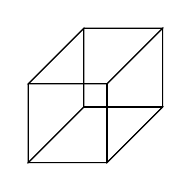
\begin{tikzpicture}[scale=1]
\draw (0,0)--(1,0)--(1,1)--(0,1)--cycle; 
\draw (0.707,0.707)--(1.707,0.707)--(1.707,1.707)--(0.707,1.707)--cycle; 
\draw (0,0)--(0.707, 0.707)--(0.707,1.707)--(0,1)--cycle;
\draw (1,0)--(1.707, 0.707)--(1.707,1.707)--(1,1)--cycle;
\draw (0,0)--(1,0)--(1.707, 0.707)--(0.707,0.707)--cycle;
\draw (0,1)--(1,1)--(1.707, 1.707)--(0.707,1.707)--cycle; \end{tikzpicture}

\newpage

\noindent Let $p$ be a fixed prime, and let $K$ run through the $S_4$-quartic fields in which $p$ does not ramify, fields being ordered by the size of the discriminants.  Then the Artin symbol takes values:
$$ \left( \frac{K_{24}}{p}\right)
= \Big[\langle e \rangle 
,\, \big\langle (12) \big\rangle
,\, \big\langle (123) \big\rangle
,\, \big\langle (1234) \big\rangle
,\, \big\langle (12)(34) \big\rangle \Big] = [\,1:6:8:6:3\,]$$
{\color{orange!50!green}\textbf{Why does everyone pretend this is settled}}\textbf{ ??} Why do Abstract Algebra teachers pretend we know how to do Galois Theory, when we can do little more than recite the insolvability of the quintic. \\ \\
In any case, we could conjecture the splitting type of a prime $p$ in a quartic field, could be proven using geometry-of-numbers in the same way that we should that $p = 4k+1 $ implies $p = a^2 + b^2 = (a+bi)(a-bi)$. There could be examples of descent.

\begin{thebibliography}{} 
\item John W. Jones, David P. Roberts \textbf{A database of number fields} \texttt{arXiv:1404.0266}
\item Manjul Bhargava, Piper Harron. \textbf{The equidistribution of lattice shapes of rings of integers in cubic, quartic, and quintic number fields} \texttt{ arXiv:1309.2025}
\item Manjul Bhargava \\
\textbf{A positive proportion of plane cubics fail the Hasse principle} \texttt{arXiv:1402.1131}
\textbf{The density of discriminants of quartic rings and fields} Volume 162, Issue 2, 1031-1063 (2005)
\item M. Bhargava, J. E. Cremona, T. A. Fisher, N. G. Jones, J. P. Keating \textbf{What is the probability that a random integral quadratic form in n variables has an integral zero?} \texttt{arXiv:1502.05992}
\end{thebibliography}  
\end{document}